\documentclass[12pt]{article}

% Packages
\usepackage{amsmath}
\usepackage{graphicx}
\usepackage[margin=0.5in, footskip=0.1in]{geometry}
\usepackage{multicol}
\usepackage{enumitem} % For itemize spacing control
\usepackage{titlesec} % For sections spacing control
\usepackage{xspace}

\begin{document}
\newgeometry{top=1in, left=0.5in, right=0.5in, bottom=0.5in, footskip=0.1in}
   \begin{center}
    \vspace{1.5cm}
    \vfill
       \Huge
       \textbf{CIFAR-10 Classification Coursework}

       \vspace{0.5cm}
       \LARGE
       ECS6P9U - Neural Networks and Deep Learning
        
       \large
       \vspace{0.5cm}
       \textbf{Christian Juresh} - 210517307
       \vspace{1.5cm}
   \end{center}
\section{Dataset and Dataloaders: 5\%}

Two sets of transformations are defined: one for dataset augmentation (used for the training dataset) and one for standard processing (used for the validation and testing datasets). To prevent overfitting, the dataset augmentation transformation includes several steps to artificially increase the diversity of the training data:

\begin{itemize}
\item \textbf{RandomHorizontalFlip:} Mirrors images horizontally at random.

\item \textbf{RandomCrop:} Randomly crops the images and adds padding.

\item \textbf{ToTensor:} Converts the images to PyTorch tensors.

\item \textbf{Cutout:} Uses my custom implementation of a random masking technique that "cuts out" one or more rectangular patches from the input image. 

\item \textbf{Normalize:} Standardises the colors of the images.
\end{itemize}
The testing dataset only includes the ToTensor and Normalize transformations. This is so that the model is tested on the original images for accurate results. DataLoaders are set up for both training and testing datasets with a batch size of 64. This gives a balance of speed and accuracy.

\section{Model: 40\%}
\subsection{Block}
The \texttt{Block} class represents one instance of many blocks, which are responsible for a sequence of operations that map an input tensor to a transformed output. It uses an \texttt{AdaptiveAvgPool2d} layer to perform spatial averaging, reducing each channel to a vector of \(d\). This vector is then transformed by a \texttt{Linear} layer, which outputs a vector \( a \) of length \( K \), the number of convolutional layers, where each element is a weight. The convolutional layers consist of a \texttt{Conv2d} layer, batch normalization, and a non-linear \texttt{ReLU} activation function. In the forward pass, a weight vector \( a \) is calculated from the linear layer's output, softmax is applied to obtain a distrubtion of weights, and the outputs of the convolutional layers are combined based on these weights to produce a single tensor \( O \). 

\restoregeometry
\subsection{Backbone}
The \texttt{Backbone} class is responsible for constructing \( N \) Blocks and their convolutional layers. It does this by sequentially stacking multiple different Block instances in two for loops,  

\subsection{Classifier}
The \texttt{Classifier} class creates a classifier that takes the output from the final Block in the Backbone and computes a mean feature vector by applying a SpatialAveragePool. This mean feature vector is then passed to a multi-layer perceptron (MLP) classifier, consisting of one fully connected layer, \texttt{ReLU} activation, dropout for regularization, and then another fully connected layer.

\subsection{Model}
The \texttt{Model} class combines the Backbone and Classifier to create a Convolutional Neural Network (CNN). The forward pass puts tensor \( X \) through the Backbone, recieves the \( O_N \) output from the \( N_{\text{th}} \) Block, and then puts it through the Classifier. 

\section{Loss and Optimizer: 5\%}
\texttt{CrossEntropyLoss} is used as the loss function. It applies a softmax function to the output of the network to compute probabilities, and then calculates the loss between the predicted probabilities and the true class labels. \texttt{optim.Adam} is used as the optimizer. It changes the learning rate and decay of the weights to reduce losses. By calculating the gradient of the loss function with respect to each weight in the model (backpropagation), the weights can be adjusted in the opposite direction of the gradient to minimize the loss. Adams optimiser is used specifically as it is fast and accurate.

\section{Training Script: 30\%}
The majority of the code in this section is for collecting metrics. The trianing script itself is quite simple. 

\subsection{Training Loop}
The training loop initializes training variables and iterates over the number of epochs to train the model. \texttt{num\_epochs} defines how many times the entire dataset will be passed through the model. For each epoch, the \texttt{train\_epoch} function is called with the \textit{model, training data loader, optimizer, loss criterion,} and \textit{device}. After each epoch, \texttt{lr\_scheduler.step} is called to adjust the learning rate based on the number of epochs.

\subsubsection{Function \texttt{train\_epoch}}
The \texttt{train\_epoch} function begins by setting the model to training mode. It iterates through the \textit{loader}, which provides batches of \textit{inputs} and their \textit{labels}. The data is then moved to the correct device.\\ \texttt{optimizer.zero\_grad} clears any old gradients from the last step so that they dont accumulate. Then the model computers the predicition for the input data. \texttt{criterion} calculates the difference between the models predicitions and the actual labels, and produces a scalar value to represent the model's performance. \texttt{loss.backward} computes the gradient of the loss with respect to the model's parameters, which are then used to adjust and update the weights with \texttt{optimizer.step}

\newpage
\subsection{Hyperparameters}
\fontsize{10}{12}\selectfont
% Reduce space around sections
\titlespacing*{\subsubsection}{0pt}{1ex plus 1ex minus .2ex}{1ex plus .2ex}

% Tighten spacing for itemize
\setlist[itemize]{topsep=0pt, partopsep=0pt, parsep=0pt, itemsep=1pt}

\begin{multicols}{2}
\subsubsection*{Dataset Augmentation Transformation}

\begin{itemize}
  \item \textbf{RandomHorizontalFlip}
    \begin{itemize}
      \item Probability: 0.5 (default)
    \end{itemize}
  \item \textbf{RandomCrop}
    \begin{itemize}
      \item Size: 32
      \item Padding: 4
    \end{itemize}
  \item \textbf{Cutout}
    \begin{itemize}
      \item Number of holes (\texttt{n\_holes}): 1
      \item Length of each hole (\texttt{length}): 16
    \end{itemize}
  \item \textbf{Normalize}
    \begin{itemize}
      \item Mean \& SD: $(0.5, 0.5, 0.5)$
    \end{itemize}
\end{itemize}

\subsubsection*{DataLoader}

\begin{itemize}
  \item Batch Size: 64
\end{itemize}

\subsubsection*{Block}

\begin{itemize}
  \item \textnumero \xspace of Convolutional Layers (\texttt{num\_convs}): Variable
  \item Kernel Size: Variable (default is 3)
  \item Padding: \texttt{kernel\_size // 2}
\end{itemize}

\subsubsection*{Backbone}

\begin{itemize}
  \item Number of Blocks (\texttt{num\_blocks}): Array of the number of Blocks in each segment of the Backbone
\end{itemize}

\subsubsection*{Classifier}

\begin{itemize}
  \item Hidden Features: \texttt{in\_features * 2}
  \item Dropout Rate: 0.5
\end{itemize}

\subsubsection*{Training Configuration}

\begin{itemize}
  \item Number of Epochs: 50
  \item Learning Rate (LR): 0.001
  \item Weight Decay: $1 \times 10^{-4}$
  \item Step Size for LR Scheduler: 30
  \item Gamma for LR Scheduler: 0.1
\end{itemize}

\subsubsection*{Model Configuration}

\begin{itemize}
  \item Number of Classes (\texttt{num\_classes}): 20
  \item In Channels: 3 (RGB)
\end{itemize}
\end{multicols}
\fontsize{12}{12}\selectfont
\subsection{Plot}
\vspace{-1cm}
\begin{center}
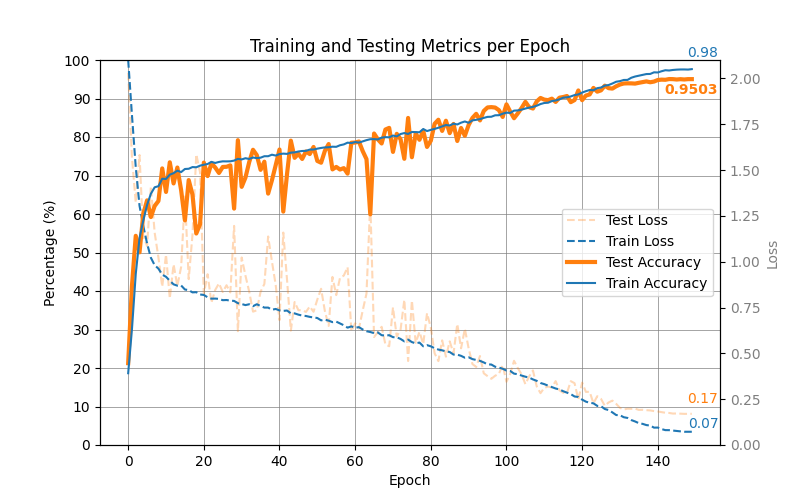
\includegraphics[width=\textwidth]{metrics.png}
\end{center}

\section{Final Model Accuracy: 20\%}
Consistently 90\% to 91\% accuracy on the test set. See plot above with 91.0700\% Test Accuracy

\end{document}